\documentclass[12pt,fleqn]{article}

\usepackage[paper]{ets-papers}
\setcounter{page}{1}

\input m-defs
\def\TN{450052}
\input colordvi

\title{
  An EMTP Theory Book Correction
}
\author{
  \vbox{\hsize=5.0in \baselineskip=12pt
    E.~T.~Scharlemann
  }
\\Lawrence Livermore National Laboratory
\\Livermore, California 94550
}

\begin{document}

%\topmargin-1in
%\oddsidemargin-1in
%\evensidemargin-1in
%\textheight792pt
%
%\includegraphics[0,0][612,792]{DC-EMTP.ps}
%\thispagestyle{empty}
%
%%\newpage
%%\thispagestyle{empty}


%\topmargin30pt
%\oddsidemargin0in
%\evensidemargin0in

\showllnl
\maketitle
\setcounter{page}{1}

In Carsons' 1926 article ~\cite{Carson} on wave propagation on a wire above the ground, the impedance of an overhead wire or pair of wires with ground return is derived, and expressed in terms of the integral
\[
   J(p, q) = P + i Q = \int_0^\infty \left( \sqrt{\mu^2 + i} - \mu \right) e^{-p\mu} \cos q\mu \; d\mu
\]
with
\[
   r = a = \sqrt{p^2 + q^2}  \ ,
\]
\[
   \theta = \phi = \tan^{-1}(q/p)  \ .
\]

The EMTP Theory Book~\cite{EMTP}, pp.~4-7  to 4-9, presents the equations stated to be used by the Alternative Transients Program ATP (or Electromagnetic Transients Program EMTP) for this impedance. The impedance expressions in~\cite{EMTP} are not the same as the expressions in~\cite{Carson}, although they are supposed to be. The main correction required to bring~\cite{EMTP} into agreement with~\cite{Carson} is to replace
\[
   \sgn = (-1)^{\left[\frac{n - 1}{4} \bmod 2\right]} = 1,1, -1, -1, -1, -1, 1, 1\ldots \text{   for   } n = 3, 4, 5, 6, 7, 8, 9, 10 \ldots
\]
as described just below Eq.~(4.12) of~\cite{EMTP}, with
\[
   \sgn = (-1)^{\left[\frac{n + 1}{2} \bmod 2\right]} = 1,1, -1, -1, 1, 1, -1, -1\ldots \text{   for   } n = 3, 4, 5, 6, 7, 8, 9, 10 \ldots  \ ;
\]
i.e., the sign of the terms in the series for $b$ alternates every two terms rather than every four terms.

The expressions in~\cite{EMTP} should be:
\[
   b_1 = \frac{\sqrt{2}}{6}
\]
\[
   b_2 = \frac{1}{16}
\]
\[
   b_n = \frac{\sgn}{n(n + 2)} b_{n - 2}
\]
\[
   c_2 = 1.3659315 = \ln \frac{2}{\gamma} + 1 + \frac{1}{2} - \frac{1}{4}
\]
($\gamma$ is defined in~\cite{Carson} as 1.7811 and is Euler's constant [$\gamma_E = 0.57722$] exponentiated: $\gamma = e^{\gamma_E}$)
\[
   c_n = c_{n-2} + \frac{1}{n} + \frac{1}{n + 2}
\]
\[
   d_n = \frac{\pi}{4} b_n
\]
\[
   \sgn = (-1)^{\left[\frac{n + 1}{2} \bmod 2\right]} = 1,1, -1, -1, 1, 1, -1, -1\ldots \text{   for   } n = 3, 4, 5, 6, 7, 8, 9, 10 \ldots \ .
\]

Other corrections are simple typographic errors, and have been caught in other references~\cite{Wang} to Carson's formula. With corrections in red, the  expressions for Carson's $P$ and $Q$ in~\cite{EMTP} should be
\begin{align*}
   P = & \frac{\pi}{8} - b_1 a \cos\phi \\
    & + b_2 \left[ (c_2 - \ln a) a^2 \cos 2\phi + \Red{\phi}\; a^2 \sin 2\phi \right] + b_3 a^3 \cos 3\phi  - d_4 a^4 \cos 4\phi - b_5 a^5 \cos 5\phi \\
    & + b_6 \left[ (c_6 - \ln a) a^6 \cos 6\phi + \phi\; a^6 \sin 6\phi \right] + b_7 a^7 \cos 7\phi  - d_8 a^8 \cos 8\phi - b_9 a^9 \cos 9\phi \\
    & + b_{10} \left[ (c_{10} - \ln a) a^{10} \cos 10\phi + \phi\; a^{10} \sin 10\phi \right] + b_{11} a^{11} \cos 11\phi  \\
    & \text{\hskip20mm} - d_{12} a^{12} \cos 12\phi - b_{13} a^{13} \cos 13\phi \ldots
\end{align*}
repeating in groups of four.
\begin{align*}
   Q = & \frac{1}{2}(0.6159315 - \ln a) + b_{\Red{1}} a \cos\phi - d_2 a^2 \cos 2\phi + b_3 a^3 \cos 3\phi \\
    & - b_4 \left[ (c_4 - \ln a) a^4 \cos 4\phi + \phi a^4 \sin 4\phi \right] + b_5 a^5 \cos 5\phi  - d_6 a^6 \cos 6\phi + b_7 a^7 \cos 7\phi \\
    & - b_8 \left[ (c_8 - \ln a) a^8 \cos 8\phi + \phi a^8 \sin 8\phi \right] + b_9 a^9 \cos 9\phi  - d_{10} a^{10} \cos 10\phi + b_{11} a^{11} \cos 11\phi \\
    & - b_{12} \left[ (c_{12} - \ln a) a^{12} \cos 12\phi + \phi a^{12} \sin 12\phi \right] + b_{13} a^{13} \cos 13\phi  \\
    & \text{\hskip20mm} - d_{14} a^{14} \cos 14\phi + b_{15} a^{15} \cos 15\phi \ldots
\end{align*}
also repeating in groups of four. The term 0.6159315 is $1/2 + \log(2/\gamma)$, and the $P$ and $Q$ are the terms inside the curly brackets of Eq.~(4.11) of~\cite{EMTP}. The typographical errors above were corrected in~\cite{Wang} but not the ordering of signs in the $b$ series.

For reference, Carson's equations~\cite{Carson} are (with $r = a$ and $\theta = \phi$):
\[
   s_2 = \frac{1}{1!2!} \left(\frac{r}{2}\right)^2 \cos 2\theta
    -\frac{1}{3!4!} \left(\frac{r}{2}\right)^6 \cos 6\theta
    +\frac{1}{5!6!} \left(\frac{r}{2}\right)^{10} \cos 10\theta \ldots
\]
\[
   s_2^\prime = \frac{1}{1!2!} \left(\frac{r}{2}\right)^2 \sin 2\theta
    -\frac{1}{3!4!} \left(\frac{r}{2}\right)^6 \sin 6\theta
    +\frac{1}{5!6!} \left(\frac{r}{2}\right)^{10} \sin 10\theta \ldots
\]
\[
   s_4 = \frac{1}{2!3!} \left(\frac{r}{2}\right)^4 \cos 4\theta
    -\frac{1}{4!5!} \left(\frac{r}{2}\right)^8 \cos 8\theta
    +\frac{1}{6!7!} \left(\frac{r}{2}\right)^{12} \cos 12\theta \ldots
\]
\[
   s_4^\prime = \frac{1}{2!3!} \left(\frac{r}{2}\right)^4 \sin 4\theta
    -\frac{1}{4!5!} \left(\frac{r}{2}\right)^8 \sin 8\theta
    +\frac{1}{6!7!} \left(\frac{r}{2}\right)^{12} \sin 12\theta \ldots
\]
\[
   \sigma_1 = \frac{r \cos\theta}{3} - \frac{r^5 \cos 5\theta}{3^2 5^2 7} + \frac{r^9 \cos 9\theta}{3^2 5^2 7^2 9^2 11} \ldots
\]
\[
   \sigma_3 = \frac{r^3 \cos 3\theta}{3^2 5} - \frac{r^7 \cos 7\theta}{3^2 5^2 7^2 9} + \frac{r^{11} \cos 11\theta}{3^2 5^2 7^2 9^2 11^2 13} \ldots
\]
\begin{align*}
   \sigma_2 = & \left( 1 + \frac{1}{2} - \frac{1}{4}\right) \frac{1}{1! 2!} \left(\frac{r}{2}\right)^2 \cos 2\theta \\
   & - \left( 1 + \frac{1}{2} + \frac{1}{3} + \frac{1}{4} - \frac{1}{8}\right) \frac{1}{3! 4!} \left(\frac{r}{2}\right)^6 \cos 6\theta \\
   & + \left( 1 + \frac{1}{2} + \frac{1}{3} + \frac{1}{4} + \frac{1}{5} + \frac{1}{6} - \frac{1}{12}\right) \frac{1}{5! 6!} \left(\frac{r}{2}\right)^{10} \cos 10\theta \ldots
\end{align*}
\begin{align*}
   \sigma_4 = & \left( 1 + \frac{1}{2} + \frac{1}{3} - \frac{1}{6}\right) \frac{1}{2! 3!} \left(\frac{r}{2}\right)^4 \cos 4\theta \\
   & - \left( 1 + \frac{1}{2} + \frac{1}{3} + \frac{1}{4} + \frac{1}{5} - \frac{1}{10}\right) \frac{1}{4! 5!} \left(\frac{r}{2}\right)^8 \cos 8\theta \\
   & + \left( 1 + \frac{1}{2} + \frac{1}{3} + \frac{1}{4} + \frac{1}{5} + \frac{1}{6} + \frac{1}{7} - \frac{1}{14}\right) \frac{1}{6! 7!} \left(\frac{r}{2}\right)^{12} \cos 12\theta \ldots
\end{align*}
\[
   P = \frac{\pi}{8}\left(1 - s_4\right) + \frac{1}{2} \left(\ln\frac{2}{\gamma} - \ln r\right)s_2 + \frac{\theta}{2} s_2^\prime - \frac{1}{\sqrt{2}}\sigma_1 + \frac{1}{2}\sigma_2 + \frac{1}{\sqrt{2}}\sigma_3  \ ,
\]
\[
   Q = \frac{1}{4} + \frac{1}{2} \left(\ln\frac{2}{\gamma} - \ln r\right)\left(1 - s_4\right) - \frac{\theta}{2} s_4^\prime - \frac{\pi}{8} s_2 + \frac{1}{\sqrt{2}}\sigma_1 + \frac{1}{\sqrt{2}}\sigma_3 - \frac{1}{2}\sigma_4  \ .
\]

Fig.~\ref{fig:l} compares the numerical results for $0 < r <= 10$ at  $\theta = 2\pi/3$ for the series in~\cite{Carson} with the corrected series from~\cite{EMTP}. 
\begin{figure}[H]
  \hbox{
     \includegraphics[width=3in]{carson.ps}
     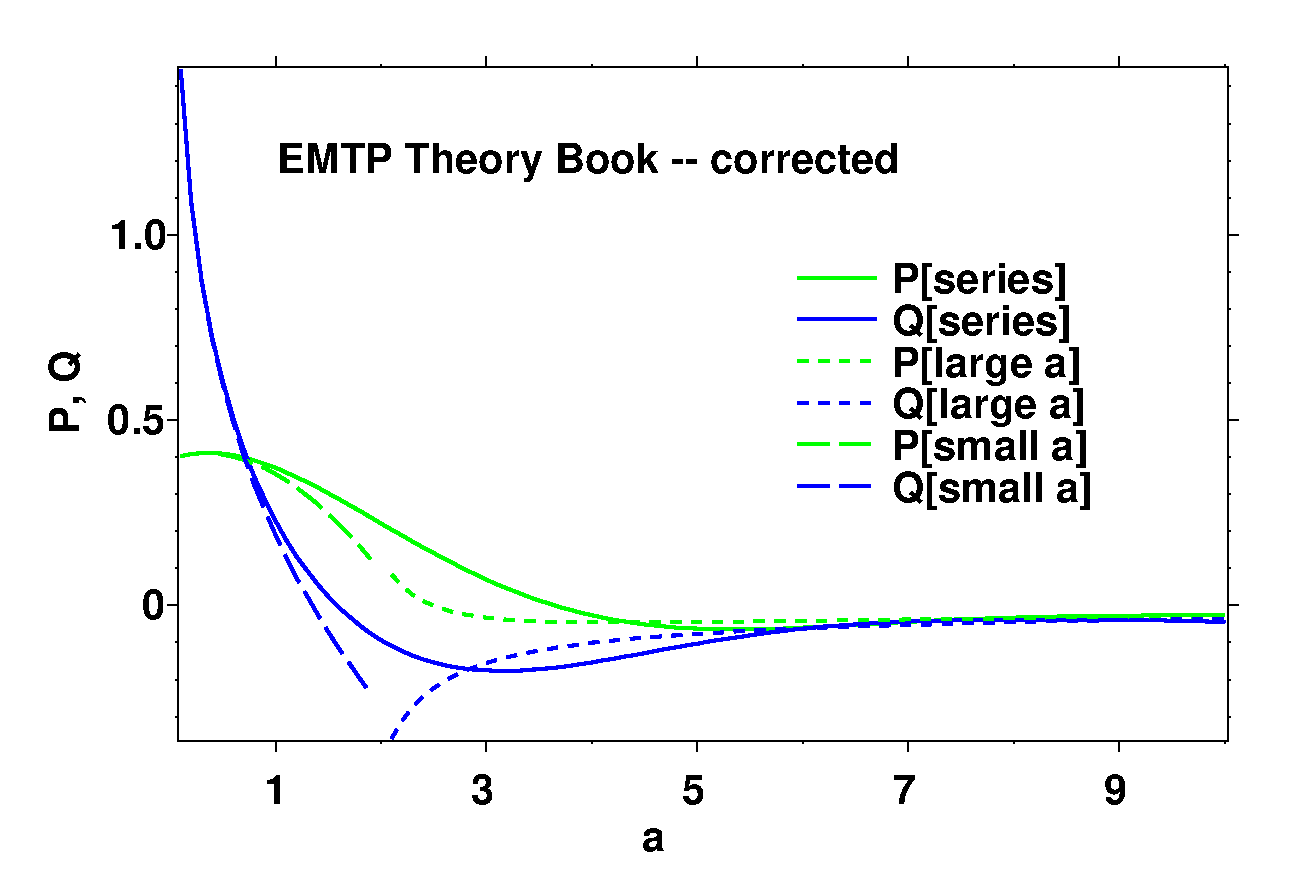
\includegraphics[width=3in]{emtp.ps}
  }
  \caption{Comparison of results for Carson's series at $\theta = 2\pi/3$ (left) and the corrected EMTP Theory Book series at the same value for $\phi$ (right). Terms up to and including $r^{23}$ (or $a^{23}$) were retained in the series to get valid results to $a = r = 10$.}
  \label{fig:l}
\end{figure}

Python programs (and typeset \LaTeX) to calculate (and display) both Carson's series and the corrected EMTP Theory Book series are available from the author.

Comparison of the corrected EMTP Theory Book series and Carson's series with the results of ATP for the impedance of a single wire above
the ground plane suggests that ATP in fact uses the correct expressions, and \emph{not} what is described in the EMTP Theory Book. Regrettably, we have been unable to obtain the source code for ATP to verify this inference.

\section*{Acknowledgments}

I am happy to acknowledge useful conversations with Barry Kirkendall and Nils Stenvig.

This work was performed under the auspices of the U.S. Department of Energy by Lawrence Livermore National Laboratory under Contract DE-AC52-07NA27344.

\vskip5mm
\baselineskip=12pt
\begin{thebibliography}{9}

\bibitem{Carson} J.~R.~Carson, ``Wave Propagation in Overhead Wires with Ground Return'', \emph{Bell System Technical Journal}, {\bf 5}, 539-554 (1926).

\bibitem{EMTP} H.~W.~Dommel, ``Electromagnetic Transients Program (EMTP) Theory Book'', Bonneville Power Administration, Portland, OR (1981 or 1986 or 1994 or ?).

\bibitem{Wang} Y.-J.~Wang and S.-J.~Liu, ``A Review of Methods for Calculation of Frequency-dependent Impedance of Overhead Power Transmission Lines,'' \emph{Proc.~Natl.~Sci.~Counc.~ROC(A)}, {\bf 25}, No.~6, pp.~329-338 (2001).

\end{thebibliography}

\vskip5mm
\hrule
\vskip5mm
\parindent=0pt

%\ets


\end{document}
